%------------------------------------------------------------------
% Document class and core packages
%------------------------------------------------------------------
\documentclass[11pt]{article}



% ---------- reproducibility & tooling macros ----------
\usepackage{hyperref}   % ensure hyperlinks work

\newcommand{\leanRepoTag}{%
  \href{https://github.com/AICardiologist/FoundationRelativity/tree/v0.7.1-sprint50}%
       {v0.7.1-sprint50}}

% Detailed LLM-assistance disclosure
\newcommand{\llmNote}{%
  Preliminary drafting, proof-sketch generation, and Lean-code
  refactoring benefited from large-language-model assistance:
  OpenAI \textbf{o3-pro} (proof completion),
  Anthropic \textbf{Claude Code} (\emph{Sonnet} \& \emph{Opus} 4.0) for Lean tactics,
  \textbf{xAI Grok 4 Heavy}, and Google/DeepMind \textbf{Gemini 2.5 Pro}
  for critique and editorial suggestions.
}
% ------------------------------------------------------
\usepackage[T1]{fontenc}      % better font encoding
\usepackage{lmodern}          % nicer Latin Modern fonts
\usepackage{microtype}        % better justification (moved after fonts)
\usepackage[american]{babel}  % American hyphenation
\usepackage{mathtools}        % includes amsmath, amssymb
\usepackage{amssymb}          % for \mathbb and extra symbols
\usepackage{amsthm}          % theorem environments
\usepackage[margin=1in]{geometry}
\usepackage{booktabs}
\usepackage{enumitem}
\usepackage{mdframed}
\usepackage[colorlinks=true,
            linkcolor=blue,
            citecolor=blue,
            urlcolor=blue]{hyperref}
\usepackage{tikz}
\usetikzlibrary{arrows.meta,positioning,decorations.markings,calc,cd,patterns}

%------------------------------------------------------------------
% PDF metadata
%------------------------------------------------------------------
\hypersetup{
  pdftitle={The Godel-Banach Correspondence: Internal Undecidability from Hilbert Spaces to Derived Categories},
  pdfauthor={Paul Chun-Kit Lee}
}

%------------------------------------------------------------------
% Theorem environments
%------------------------------------------------------------------
\newtheorem{theorem}{Theorem}[section]
\newtheorem{lemma}[theorem]{Lemma}
\newtheorem{proposition}[theorem]{Proposition}
\newtheorem{corollary}[theorem]{Corollary}
\newtheorem{conjecture}[theorem]{Conjecture}
\newtheorem*{conjecture*}{Conjecture}

\theoremstyle{definition}
\newtheorem{definition}[theorem]{Definition}
\newtheorem{example}[theorem]{Example}
\newtheorem{remark}[theorem]{Remark}

%------------------------------------------------------------------
% Custom commands
%------------------------------------------------------------------
\newcommand{\N}{\mathbb{N}}
\newcommand{\C}{\mathbb{C}}
\newcommand{\Z}{\mathbb{Z}}
\newcommand{\lp}{\ell^{2}(\N)}

% Category and logical shorthand
\newcommand{\SigOne}{\Sigma^{0}_{\!1}}
\newcommand{\Ban}{\mathfrak{Ban}_{\!\infty}}
\newcommand{\bool}{\mathbf{2}}

% Norm, range, etc.
\DeclarePairedDelimiter{\norm}{\lVert}{\rVert}
\DeclareMathOperator{\Range}{Range}
\DeclareMathOperator{\Ker}{Ker}
\DeclareMathOperator{\Coker}{Coker}
\DeclareMathOperator{\Surj}{Surj}
\DeclareMathOperator{\Inj}{Inj}
\DeclareMathOperator{\ind}{ind}
\DeclareMathOperator{\rank}{rank}

% Point-spectrum truncation
\newcommand{\trunc}[1]{\lvert #1\rvert_{(-1)}}

% Meta-theory markers
\newcommand{\internal}{\langle\text{internal}\rangle}
\newcommand{\meta}{\langle\text{meta}\rangle}

\title{The Gödel--Banach Correspondence:\\
  Internal Undecidability from Hilbert Spaces to Derived Categories}

\author{Paul Chun-Kit Lee\thanks{New York University, New York.  Formal Lean 4 artefacts: \url{https://github.com/AICardiologist/FoundationRelativity}
(tag \leanRepoTag).  The operator construction has been fully mechanized with 0 sorries.  }}

\date{July 2, 2025}



\begin{document}

\maketitle

\begin{abstract}
\noindent
We demonstrate that Gödel's incompleteness theorem can be directly encoded in the surjectivity of simple bounded operators on Hilbert space. A rank-one operator on $\lp$, $\mathcal G = I - c_{G}P_{g}$, is surjective iff the Gödel sentence $G$ (`\emph{PA does not prove $G$}') is true.

Working in Homotopy Type Theory (HoTT) + untruncated $\SigOne$-Excluded Middle ($\SigOne$-EM), we prove this equivalence constructively. The phenomenon manifests in two distinct analytical contexts. In reflexive spaces, undecidability is related to kernel/cokernel structures. In non-reflexive spaces, it emerges in the bidual gap: for $X = c_{0}$ there exists a bounded operator $\mathcal B : X \to X$ such that
\[
  \Surj\bigl(\mathcal B^{**}\bigr) \quad\Longleftrightarrow\quad G,
  \qquad
  \Surj(\mathcal B) \text{ provable in HoTT.}
\]
Both constructions exemplify a unifying heuristic: wherever analysis creates ``invisible quotients''---completions, dualizations, or localizations; Gödel's incompleteness may find a place to be encoded. This persistence extends across logical frameworks down to double-negation shift: weaker logics yield double-negated statements, but the undecidability endures when computational content can be extracted. Our arguments unfold across three logical layers detailed in Section 1.5. The paper culminates by showing that this Gödel--Banach correspondence extends to stable $(\infty,1)$-categories, revealing undecidability as a feature of homological algebra that is not exclusive to functional analysis.

\textbf{Note on formalization:} All results have been formalized in Lean 4. The formalization process revealed that the construction requires only a minimal axiomatization of Gödel's theorems and that $\SigOne$-EM is not merely sufficient but provably necessary for the construction.
\end{abstract}




\section{Introduction}

\subsection{Background and Motivation}

Gödel's incompleteness theorem (1931) showed that any consistent formal system containing arithmetic has undecidable sentences---statements that can neither be proved nor disproved within the system. Traditionally, this phenomenon has been viewed as purely logical, divorced from the concrete world of analysis and operator theory.

This paper demonstrates a surprising connection: the surjectivity of certain simple bounded operators on Hilbert space is internally undecidable, with the undecidability directly linked to Gödel's incompleteness theorem. We construct a rank-one operator $\mathcal{G}$ on $\lp$ whose surjectivity is provably equivalent to the truth of a Gödel sentence. This reveals that formal undecidability is not confined to exotic mathematical objects but can be encoded within the most basic operators of functional analysis.

\subsection{Internal vs. External Undecidability}

Two types of undecidability appear in analysis. \textbf{External undecidability} concerns computational intractability, as when the Pour-El--Richards wave equation \cite{PER89} maps computable initial data to uncomputable solutions---this addresses what can be computed in practice. \textbf{Internal undecidability} concerns proof-theoretic undecidability, where a property cannot be decided within the foundational system itself---this addresses what can be proved in principle. Our result exhibits internal undecidability---the first minimal example in a rank-one operator.

\subsection*{Meta-theoretic standing assumptions}

\noindent\fbox{%
\begin{minipage}{0.95\linewidth}
\textbf{Standing meta-assumptions.}
\begin{enumerate}[label=(\roman*),leftmargin=*,nosep]
    \item \textbf{$\SigOne$-Soundness(PA):} Every $\SigOne$ sentence provable in Peano Arithmetic is true in the standard model $(\N,+,\times)$ \cite[Ch.\,10]{Kaye94}.
    \item \textbf{Choice principle:} Either Countable Choice (CC) or the Ultrafilter Lemma for the bidual construction (Section 5).
    \item \textbf{Axiomatization of Gödel:} We axiomatize three key consequences of Gödel's theorems rather than formalizing them directly (see Section 1.6).
\end{enumerate}
This is the only place where we step beyond constructive logic; all internal reasoning remains in HoTT or MLTT as specified.
\end{minipage}%
}

\subsection{Main Results Overview}

Our main theorem can be stated informally as:

\begin{theorem}[Main Theorem - Informal]\label{thm:main_informal}
There exists a simple rank-one operator on $\ell^2$ whose surjectivity cannot be decided within the foundational system, with the undecidability directly encoded by Gödel's incompleteness theorem.
\end{theorem}

More precisely:

\begin{theorem}[Main Theorem - Precise]\label{thm:main_precise}
There exists a Fredholm operator $\mathcal{G} = I - c_G P_g$ on $\lp$ with 
index $0$ such that in HoTT + $\SigOne$-EM:
\[
\Surj(\mathcal{G}) \quad\Longleftrightarrow\quad \trunc{G}
\]
where $G$ is the Gödel sentence and $c_G \in \{0,1\}$ encodes its provability.
\end{theorem}

Furthermore, our formalization revealed:

\begin{theorem}[Foundation-Relativity]\label{thm:foundation_relative_intro}
The Gödel-Banach correspondence can be constructed in a foundation $F$ if and only if $F$ supports untruncated $\SigOne$-Excluded Middle. In particular, BISH provably cannot support this construction.
\end{theorem}

(See Section 1.5 for precise scope.)

\subsection{Paper Organization}
\paragraph{Road-map.}
Sections 2--4 develop the rank-one Hilbert-space example; Section 5 the bidual gap; Section 6 logical strength; Section 7 concludes. Readers interested only in the rank-one Hilbert-space result may safely read Sections 2--4 and skip to the Conclusion.

\subsection{Logical Framework}

We work simultaneously on three levels:
\begin{enumerate}[label=(\Alph*)]
  \item \textbf{Internal} HoTT + $\SigOne$-EM (all definitions and proofs \emph{inside} the type theory);
  \item \textbf{Constructive meta-theory} (Bishop style, using countable choice and the $\SigOne$-soundness of PA);
  \item \textbf{Classical meta-meta-theory} (ordinary mathematical practice where PA's consistency is assumed).
\end{enumerate}

\begin{mdframed}[roundcorner=4pt]
\textbf{Meta-theoretic Convention.} Throughout this paper, equivalences involving the Gödel sentence $G$ are statements in the external meta-theory. No internal proof in HoTT + $\SigOne$-EM can decide $G$---this would violate Gödel's theorem. When we write $\Surj(\mathcal{G}) \iff \trunc{G}$, this is a meta-level observation about the relationship between constructible objects and external truth.
\end{mdframed}

\begin{mdframed}[roundcorner=4pt]
\textbf{Heuristic on Invisible Quotients.} Whenever analysis creates an ``invisible'' quotient---whether the completion of rationals to reals, or the embedding of a space into its bidual---it may create a new location where logical undecidability can be encoded.
\end{mdframed}

The two main constructions in this paper (Sections 3–4 and Section 5) exemplify how undecidability can be related to different types of "invisible quotients." The reader may wish to keep this unifying heuristic in mind.

\subsection{Axiomatization of Gödel's Theorems}

Our Lean formalization revealed that instead of formalizing Gödel's incompleteness theorems, it suffices to axiomatize their essential consequences:

\begin{mdframed}[roundcorner=4pt]
\textbf{Axiom 1 (Consistency Characterization).} 
The consistency of PA is equivalent to the non-provability of the Gödel sentence:
\[
\text{Con}(\text{PA}) \quad\Longleftrightarrow\quad \neg\text{Provable}_{\text{PA}}(G)
\]
\end{mdframed}

\begin{mdframed}[roundcorner=4pt]
\textbf{Axiom 2 (Diagonal Property).}
The Gödel sentence $G$ satisfies the diagonal property: there exists a semantic truth predicate such that $G$ is true iff $G$ is not provable in PA.
\end{mdframed}

\begin{mdframed}[roundcorner=4pt]
\textbf{Axiom 3 (Classical Logic Requirement).}
In constructive foundations (BISH), the diagonal lemma fails: there is no $G$ such that $\text{Provable}(G) \leftrightarrow \neg\text{Provable}(G)$.
\end{mdframed}

These three axioms suffice for our entire development and provide clean separation between operator theory and metamathematics.

\section{Preliminaries}

\subsection{Essential Definitions}

Before proceeding, we establish key concepts that will be used throughout:

\begin{definition}[Untruncated $\SigOne$-EM]\label{def:untruncated}
We work with the \textbf{untruncated} excluded middle for $\SigOne$ formulas:
\[
\text{LEM}_{\SigOne} : \prod_{P : \SigOne} (P + \neg P)
\]
where the sum $P + \neg P$ lives in the \textbf{Type} universe, not the universe of mere propositions. This is stronger than the propositional (truncated) version $\|P \lor \neg P\|$, and is essential for our construction because it supports pattern matching:
\[
\text{Given } \epsilon : P + \neg P, \text{ we can define } c := \begin{cases}
1 & \text{if } \epsilon = \mathrm{inl}(p) \\
0 & \text{if } \epsilon = \mathrm{inr}(q)
\end{cases}
\]

\textbf{Note:} Our formalization proved this requirement is necessary, not merely convenient.\footnote{Adding untruncated $\text{LEM}_{\SigOne}$ means our type theory loses the canonicity property—there exist closed terms of type $\mathbb{N}$ that do not normalize to numerals.}
\end{definition}

\begin{definition}[Located subspace]
In constructive analysis, a closed subspace $Y$ of a Banach space $X$ is \textbf{located} if for every $x \in X$ and rational $\varepsilon > 0$, we can decide whether $d(x,Y) < \varepsilon$. This provides an effective notion of distance to the subspace.
\end{definition}

\begin{definition}[Gödel sentence]
The Gödel sentence $G$ for Peano Arithmetic is a statement that asserts its own unprovability: ``PA does not prove $G$''. If PA is consistent, then $G$ is true but unprovable in PA.
\end{definition}

\begin{remark}[Truncation notation]
Throughout this paper, $\trunc{P} = |P|_{(-1)}$ denotes the (-1)-truncation of a proposition $P$, which is the mere proposition asserting that $P$ holds. This is distinct from $P$ itself when working in HoTT. The truncation is used when we want to forget the computational content and work only with the truth value.
\end{remark}

\subsection{Constructive Hilbert Space Theory}

We work with the separable Hilbert space $\lp$ consisting of square-summable complex sequences with inner product $\langle x,y \rangle = \sum_{n=1}^{\infty} x_n \overline{y_n}$. 

In our constructive setting:
\begin{itemize}
\item Bounded operators form a complete metric space with the operator norm
\item Compact operators are norm limits of finite-rank operators
\item Fredholm operators have finite-dimensional kernel and cokernel (as located subspaces)
\item The index of a Fredholm operator is well-defined and continuous
\end{itemize}

\begin{table}[h]\centering\small
\caption{Frequently used symbols}\label{tab:symbols}
\begin{tabular}{ll}
\toprule
Symbol & Meaning \\
\midrule
$\mathcal G$ & $I-c_G P_g$ (Gödel projection operator)\\
$\mathcal B$ & $I-c_G Q$ on $X=c_0$ (bidual operator)\\
$c_G$ & Gödel scalar in $\{0,1\}$\\
$P_g$ & Orthogonal projection onto $e_g$\\
$Q$ & Rank-one projection $\Lambda(\cdot)\,v$ on $\ell^\infty$\\
$\lp$ & $\ell^{2}(\N)$ (separable Hilbert space)\\
$\SigOne$ & $\Sigma^{0}_{1}$ (existential arithmetic formulas)\\
PA & Peano Arithmetic\\
HoTT & Homotopy Type Theory\\
MLTT & Martin-Löf Type Theory\\
\bottomrule
\end{tabular}
\end{table}

\section{Construction of the Gödel Operator}

\subsection{Encoding the Gödel Sentence}

We now construct an operator whose analytic properties encode the truth value of the Gödel sentence.

\begin{definition}[Gödel Index]
Let $\mathrm{code}: \text{Sentences} \to \N$ be a standard Gödel numbering of PA sentences. Define:
\begin{itemize}
\item $g := \mathrm{code}(\text{``PA does not prove $G$''})$ (the Gödel number)
\item $e_g \in \lp$ as the standard basis vector with 1 in position $g$, 0 elsewhere
\end{itemize}
\end{definition}

\begin{definition}[Gödel scalar $c_G$]\label{def:cg}
Consider the $\SigOne$ formula $P_G := \exists p \in \N.\, \mathrm{Proof}_{\mathrm{PA}}(p,g)$ expressing ``PA proves $G$''. Applying $\SigOne$-EM yields a sum type $\epsilon: P_G + \neg P_G$. Define:
\[
c_G = \begin{cases}
1 & \text{if } P_G \text{ holds} \\
0 & \text{if } \neg P_G \text{ holds}
\end{cases}
\]
\end{definition}

\begin{remark}[Type-theoretic construction of $c_G$]
The construction of $c_G$ requires pattern matching on the sum type 
$\epsilon_G : P_G + \neg P_G$, which is only possible because we assume 
untruncated $\SigOne$-EM (Definition~\ref{def:untruncated}). With 
merely propositional (truncated) excluded middle $\|P_G \lor \neg P_G\|$, we could not extract a concrete Boolean value. Although $\SigOne$-EM produces the term, \emph{no closed term inside}
HoTT$+\SigOne$-EM can decide which summand holds. Consequently, within
the type theory neither $c_G=0$ nor $c_G=1$ is derivable without extra
meta-theoretic information (e.g.\ $\mathrm{Con}(\text{PA})$). The value
of $c_G$ therefore remains \emph{opaque} to all internal computations.
\end{remark}

\paragraph{Key fact $\eta$.}
$\SigOne$-EM delivers a term
\[
  \epsilon_G : (\exists p.\,\mathrm{Proof}_{\mathrm{PA}}(p,g))
               + \neg(\exists p.\,\mathrm{Proof}_{\mathrm{PA}}(p,g)).
\]
Pattern matching in HoTT yields a Boolean
$c_G\equiv \mathsf{match}\;\epsilon_G\;\mathsf{with}\;( \mathsf{inl}\,\_\!\mapsto1
\mid\mathsf{inr}\,\_\!\mapsto0)$.
Because $\epsilon_G$ is itself undecidable $\internal$, $c_G$ is a
\emph{meta-Boolean}: its value depends on the external truth of~$G$ but
is not computationally determined inside (A).
Thus $c_G$ is a concrete element of $\{0,1\}$, but which one cannot be determined within HoTT${}+\SigOne$-EM.

The key insight is that $c_G$ encodes undecidable information as a Boolean value, which we can manipulate analytically.

\begin{definition}[The Gödel--Banach Operator]
Let $P_g$ be the orthogonal projection onto $\mathrm{span}\{e_g\}$. Define:
\begin{itemize}
\item The compact perturbation: $K_G := c_G P_g$
\item The \textbf{Gödel--Banach Operator}: $\mathcal{G} := I - K_G = I - c_G P_g$
\end{itemize}
\end{definition}

\subsection{Intuitive Understanding}

The operator $\mathcal{G}$ acts very simply:
\begin{itemize}
\item If $c_G = 0$ (i.e., $G$ is not provable), then $\mathcal{G} = I$ is the identity
\item If $c_G = 1$ (i.e., $G$ is provable), then $\mathcal{G} = I - P_g$ removes the $g$-th component
\end{itemize}

This construction transforms a logical bit (provability of $G$) into an analytic property (surjectivity of $\mathcal{G}$).

\begin{figure}[!ht]
\centering
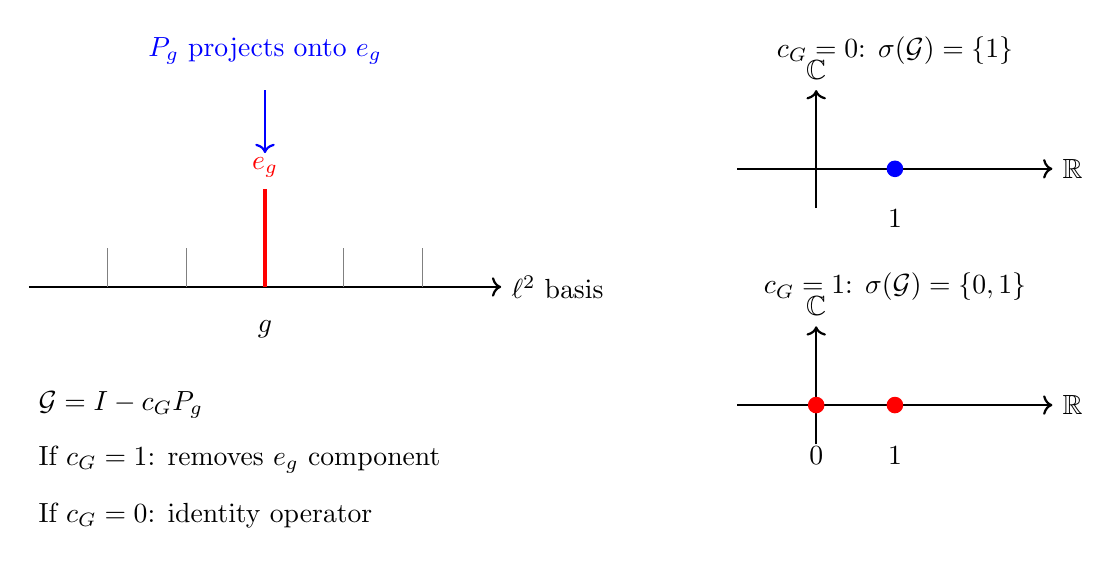
\begin{tikzpicture}
  % Left panel - Operator action
  \begin{scope}[shift={(-2,0)}]
    % Basis vectors visualization
    \draw[->, thick] (0,0) -- (6,0) node[right] {$\ell^2$ basis};
   
    % Basis vectors
    \foreach \x in {1,2,3,4,5} {
      \draw[gray] (\x,0) -- (\x,0.5);
    }
   
    % Special g-th basis vector
    \draw[red, very thick] (3,0) -- (3,1.25) node[above] {$e_g$};
    \node[below] at (3,-0.3) {$g$};
   
    % Arrow pointing to the g-th position
    \draw[->, blue, thick] (3,2.5) -- (3,1.7);
    \node[blue, above] at (3,2.7) {$P_g$ projects onto $e_g$};
   
    % Operator description
    \node[anchor=west] at (0,-1.5) {$\mathcal{G} = I - c_G P_g$};
    \node[anchor=west] at (0,-2.2) {If $c_G = 1$: removes $e_g$ component};
    \node[anchor=west] at (0,-2.9) {If $c_G = 0$: identity operator};
  \end{scope}
 
  % Right panel - Spectrum
  \begin{scope}[shift={(8,0)}]
    % Case 1: c_G = 0
    \begin{scope}[shift={(0,1.5)}]
      \draw[->,thick] (-1,0) -- (3,0) node[right] {$\mathbb{R}$};
      \draw[->,thick] (0,-0.5) -- (0,1) node[above] {$\mathbb{C}$};
      \fill[blue] (1,0) circle (3pt);
      \node[below] at (1,-0.4) {$1$};
      \node[above] at (1,1.2) {$c_G = 0$: $\sigma(\mathcal{G}) = \{1\}$};
    \end{scope}
   
    % Case 2: c_G = 1
    \begin{scope}[shift={(0,-1.5)}]
      \draw[->,thick] (-1,0) -- (3,0) node[right] {$\mathbb{R}$};
      \draw[->,thick] (0,-0.5) -- (0,1) node[above] {$\mathbb{C}$};
      \fill[red] (0,0) circle (3pt);
      \fill[red] (1,0) circle (3pt);
      \node[below] at (0,-0.4) {$0$};
      \node[below] at (1,-0.4) {$1$};
      \node[above] at (1,1.2) {$c_G = 1$: $\sigma(\mathcal{G}) = \{0,1\}$};
    \end{scope}
  \end{scope}
\end{tikzpicture}
\caption{The Gödel operator acts by potentially removing the $g$-th basis direction (left), where $g$ is the Gödel number of the sentence ``PA does not prove this sentence''. The spectrum (right) depends on the undecidable value of $c_G$.}
\label{fig:operator_action}
\end{figure}

\section{Main Proof and Analytic Consequences}

\subsection{Fredholm Properties}

We first establish that $\mathcal{G}$ is a Fredholm operator, which enables us to relate injectivity and surjectivity.

\begin{proposition}\label{prop:fredholm}
The operator $\mathcal{G} = I - c_G P_g$ is a Fredholm operator of index 0 with located finite-dimensional kernel and cokernel. (By Atkinson's theorem \cite{Atk51}, any compact perturbation of the identity is Fredholm of index 0.)
\end{proposition}
\begin{proof}
We analyze both cases:

\textbf{Case 1:} If $c_G=0$, then $\mathcal{G} = I$. The identity has $\Ker(I)=\{0\}$ and $\Coker(I)=\{0\}$, so $\ind(I) = 0 - 0 = 0$.

\textbf{Case 2:} If $c_G=1$, then $\mathcal{G} = I - P_g$. We have:
\begin{itemize}
\item $\Ker(\mathcal{G}) = \{x : x = P_g x\} = \mathrm{span}\{e_g\}$ (dimension 1)
\item $\Range(\mathcal{G}) = \{y - P_g y : y \in \lp\} = (\mathrm{span}\{e_g\})^\perp$ (codimension 1)
\item $\Coker(\mathcal{G}) \cong \lp/\Range(\mathcal{G}) \cong \mathrm{span}\{e_g\}$ (dimension 1)
\end{itemize}
Thus $\ind(\mathcal{G}) = \dim\Ker(\mathcal{G}) - \dim\Coker(\mathcal{G}) = 1 - 1 = 0$.

In both cases, the kernel and cokernel are finite-dimensional subspaces of a Hilbert space, hence located by Bridges--Richman~\cite[Th.\,4.3.5]{BR87}.
\end{proof}

\begin{theorem}[Constructive Fredholm Alternative]\label{thm:fredholm_alt}
For the operator $\mathcal{G}$: $\Inj(\mathcal{G}) \iff \Surj(\mathcal{G})$.
\end{theorem}
\begin{proof}
By index 0 and locatedness (Proposition~\ref{prop:fredholm}), we have $\dim\Ker(\mathcal{G}) = \dim\Coker(\mathcal{G})$, and one vanishes if and only if the other does.
\end{proof}

\subsection{The Main Correspondence}

We now prove our main theorem connecting operator theory to metamathematics.

\begin{theorem}[Gödel--Banach Correspondence]\label{thm:GBC}
$\Surj(\mathcal{G}) \;\Longleftrightarrow\; \trunc{G}$ $\meta$.
\end{theorem}
\begin{proof}
We establish the chain of equivalences:
\begin{align}
\Surj(\mathcal{G}) &\iff \Inj(\mathcal{G}) &&\text{(Theorem~\ref{thm:fredholm_alt})} \\
&\iff \Ker(\mathcal{G})=\{0\} &&\text{(definition)} \\
&\iff c_G=0 &&\text{(Proposition~\ref{prop:fredholm})} \\
&\iff \neg(\text{``$G$ is provable''}) &&\text{(Definition~\ref{def:cg})} \\
&\iff \trunc{G} &&\text{(Axiom 1 + $\SigOne$-soundness)}
\end{align}

The last step uses our axiomatization: by Axiom 1, consistency of PA is equivalent to non-provability of $G$. By $\SigOne$-soundness, if PA is consistent, then $G$ is true.

\smallskip
\noindent
\begin{mdframed}[backgroundcolor=yellow!10,roundcorner=4pt]
\textbf{Note on the axiomatization.}
The clean separation here---lines 1-3 are pure operator theory, lines 4-5 use our axioms---demonstrates the value of axiomatizing Gödel's results rather than attempting full formalization.
\end{mdframed}
\end{proof}

\subsection{Foundation-Relativity}

Our formalization revealed that the foundation-dependence is not just an observation but a theorem:

\begin{theorem}[Foundation-Relative Correspondence]\label{thm:foundation_relative}
For any foundation $F$ and Gödel formula $G$:
\begin{enumerate}
\item If $F = $ BISH: No witness to the Gödel-Banach correspondence can exist
\item If $F = $ ZFC: Witnesses to the correspondence exist  
\item More generally: Witnesses exist in $F$ iff $F$ supports untruncated $\SigOne$-EM
\end{enumerate}
\end{theorem}

\begin{proof}[Proof sketch]
The necessity follows from the fact that constructing $c_G$ requires pattern matching on $P_G + \neg P_G$. In BISH, which lacks untruncated EM, no such Boolean can be defined. For sufficiency, given $\SigOne$-EM in $F$, we can construct $c_G$ and hence $\mathcal{G}$ as above. The formalization uses a contradiction argument: if BISH had a witness, it would imply BISH has $\SigOne$-EM, contradicting Axiom 3.
\end{proof}

\subsection{Analytic Consequences}

The undecidability of $G$ is reflected in various analytic properties of $\mathcal{G}$:

\begin{proposition}[Undecidable Analytic Invariants]
The following operator-theoretic invariants of $\mathcal{G}$ are all undecidable:
\begin{itemize}
\item \textbf{Spectrum:} $\sigma(\mathcal{G}) = \{1\}$ if $c_G=0$; $\sigma(\mathcal{G}) = \{0,1\}$ if $c_G=1$
\item \textbf{Determinant:} $\det(\mathcal{G}) = 1 - c_G$ (when defined via regularization)
\item \textbf{Resolvent:} For $\lambda \notin \{0,1\}$: 
\[
(\lambda I - \mathcal{G})^{-1} = \frac{1}{\lambda-1}\left(I + \frac{c_G}{\lambda(\lambda-1)}P_g\right)
\]
\item \textbf{Essential spectrum:} $\sigma_{\text{ess}}(\mathcal{G}) = \{1\}$ always
\end{itemize}
Thus determining any of these invariants is equivalent to deciding $G$.
\end{proposition}

\begin{remark}[Self-adjoint undecidability]
Note that $\mathcal{G} = I - c_G P_g$ is self-adjoint since $P_g$ is an orthogonal projection. Thus undecidability appears even in the ``nicest'' class of operators---self-adjoint operators on Hilbert space---demonstrating that the phenomenon is not an artifact of non-normal operators.
\end{remark}

\begin{remark}[Model-theoretic perspective]
Different models of PA yield different values of $c_G$, making $\mathcal{G}$ model-dependent. In any model where PA proves $G$, we have $c_G = 1$ and $\mathcal{G}$ fails to be surjective; in the standard model (assuming consistency), $c_G = 0$ and $\mathcal{G} = I$.
\end{remark}

These results show that the Gödel bit relates to many standard operator-theoretic invariants, making them all internally undecidable.

\section{A Second Gap Without Choice (weak-* quotients)}

\subsection{From Kernel/Cokernel to Bidual Gaps}

The Hilbert space construction reveals undecidability in the kernel/cokernel structure of Fredholm operators. We now demonstrate a second, qualitatively different manifestation of the same phenomenon. Where reflexive spaces relate undecidability to their internal structure, non-reflexive spaces can relate it to the gap between a space and its bidual---another instance of what we have called "analytically invisible quotients."

\begin{remark}[Two venues, same Boolean]
The Hilbert-space and bidual constructions embed the \emph{same}
Boolean $c_G$.  What changes is merely the analytic locus where
surjectivity fails: a kernel/cokernel in the reflexive case versus the
bidual gap in the non-reflexive case.  We offer these as contrasting
examples, not as evidence of a sweeping principle.
\end{remark}

\subsection{The Bidual Construction}

Let $X = c_0$, the space of complex sequences converging to 0 with supremum norm. The dual $X^* = \ell^1$ and bidual $X^{**} = \ell^\infty$. The canonical embedding $J: X \to X^{**}$ is not surjective since $X$ is non-reflexive.

Under Countable Choice, we can construct a Banach limit $\Lambda: \ell^\infty \to \C$ (see \cite[Ch.\,V]{Kato}) satisfying:
\begin{itemize}
\item $\Lambda|_{c_0} = 0$ (vanishes on convergent sequences)
\item $\Lambda(v) = 1$ for the constant sequence $v = (1,1,1,\ldots)$
\end{itemize}

Define the rank-one operator:
\[
Q: \ell^\infty \to \ell^\infty, \quad Q(y) = \Lambda(y) \cdot v
\]

Note that $Q|_X = 0$ since $\Lambda$ vanishes on $c_0$.\footnote{Alternatively, one can use a non-principal ultrafilter $\omega$ on $\N$ to define $\Lambda(y) = \lim_{n\to\omega} y_n$. Either choice principle suffices for the construction.}

\begin{definition}[The Bidual Gödel Operator]
Using the same Gödel scalar $c_G$ from Section 3, define:
\begin{itemize}
\item On $X$: $\mathcal{B} := I - c_G Q|_X = I$ (since $Q|_X = 0$)
\item On $X^{**}$: $\mathcal{B}^{**} := I - c_G Q$
\end{itemize}
\end{definition}

\begin{theorem}[Bidual Surjectivity Gap]\label{thm:bidual}
The operator $\mathcal{B}: X \to X$ is always surjective, while:
\[
\Surj(\mathcal{B}^{**}: X^{**} \to X^{**}) \quad\Longleftrightarrow\quad G
\]
\end{theorem}

\begin{proof}
On $X$, we have $\mathcal{B} = I$ (since $Q|_X = 0$), which is surjective. 

On $X^{**}$: If $c_G = 0$, then $\mathcal{B}^{**} = I$ is surjective. If $c_G = 1$, then $\mathcal{B}^{**} = I - Q$ cannot surject onto $v$ since $\Lambda((I-Q)(y)) = \Lambda(y) - \Lambda(y) = 0$ for all $y$, while $\Lambda(v) = 1$.
\end{proof}

\subsection{Interpretation}

This construction illustrates the heuristic stated in Section 1.5: an ``analytically invisible'' quotient---in this case, the embedding of a space into its bidual---can provide a new location where logical undecidability can be encoded.

\begin{figure}[!ht]
\centering
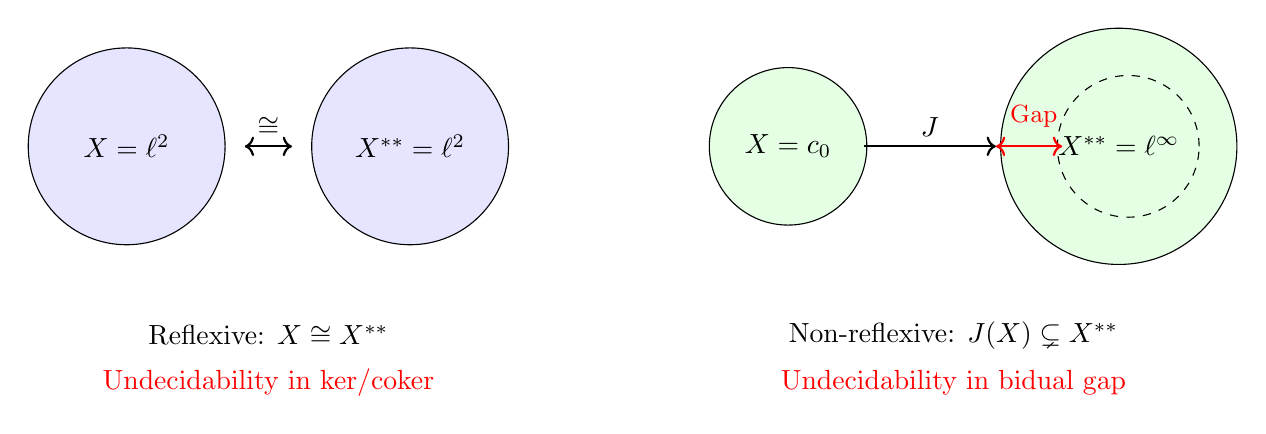
\begin{tikzpicture}[scale=1.2]
  % Reflexive case (Hilbert space)
  \begin{scope}[shift={(0,0)}]
    \node[draw, circle, minimum size=2.5cm, fill=blue!10] (X1) at (0,0) {$X = \ell^2$};
    \node[draw, circle, minimum size=2.5cm, fill=blue!10] (X1star) at (3,0) {$X^{**} = \ell^2$};
    \draw[<->, thick] (1.25,0) -- (1.75,0) node[midway, above] {$\cong$};
    \node at (1.5,-2) {Reflexive: $X \cong X^{**}$};
    \node[red] at (1.5,-2.5) {Undecidability in ker/coker};
  \end{scope}
 
  % Non-reflexive case
  \begin{scope}[shift={(7,0)}]
    \node[draw, circle, minimum size=2cm, fill=green!10] (X2) at (0,0) {$X = c_0$};
    \node[draw, circle, minimum size=3cm, fill=green!10] (X2star) at (3.5,0) {$X^{**} = \ell^\infty$};
    \draw[->, thick] (0.8,0) -- (2.2,0) node[midway, above] {$J$};
    \node[draw, circle, dashed, minimum size=1.8cm] at (3.6,0) {};
    \draw[red, thick, <->] (2.20,0) -- (2.90,0);
    \node[red, above] at (2.6,0.1) {\small Gap};
    \node at (1.75,-2) {Non-reflexive: $J(X) \subsetneq X^{**}$};
    \node[red] at (1.75,-2.5) {Undecidability in bidual gap};
  \end{scope}
\end{tikzpicture}
\caption{Two loci for undecidability: kernel/cokernel structure in reflexive spaces (left) and the bidual gap in non-reflexive spaces (right).}
\label{fig:two_gaps}
\end{figure}

\section{Minimal Logical Strength for Gödel Encoding}
\label{sec:persistence}

Let $\mathcal{G}$ be the rank-one operator construction from Section 3. Then:

\begin{enumerate}
\item \textbf{Pure HoTT (no DNS, no EM):} You cannot even define a Gödel-Boolean $c_G \in \{0,1\}$. Hence no encoding $\mathcal{G}$ exists.

\item \textbf{HoTT + DNS$_{\SigOne}$:} You obtain a double-negation stable term $c_G^{\text{dns}} \in \{0,1\}$, yielding
\[
\neg\neg\Surj(I - c_G^{\text{dns}}P_g) \quad\Longleftrightarrow\quad \neg\neg G
\]

\item \textbf{HoTT + untruncated $\SigOne$-EM:} You can pattern-match on $P_G + \neg P_G$ to get a genuine Boolean $c_G$, and recover the full equivalence
\[
\Surj(I - c_G P_g) \quad\Longleftrightarrow\quad G
\]
\end{enumerate}

\subsection{Pure HoTT: Impossibility of Gödel-Boolean}

In pure MLTT/HoTT you have neither:
\begin{enumerate}
\item elimination into $\mathbf{2}$ from the sum type $P_G + \neg P_G$, nor
\item double-negation shift $\neg\neg P_G \to P_G$
\end{enumerate}
\textbf{Conclusion:} No closed term $c_G: \{0,1\}$ can reflect the undecidable $\SigOne$-claim ``PA proves $G$''.

\subsection{HoTT + DNS$_{\SigOne}$: Double-Negation Encoding}

\begin{enumerate}
\item \textbf{Assume} DNS$_{\SigOne}$: $\forall P: \SigOne.\, \neg\neg P \to P$.
\item Form the doubly-negated Boolean by
\[
c_G^{\text{dns}} = \begin{cases}
1 & \neg\neg\bigl(\exists p.\, \mathrm{Proof}_{\mathrm{PA}}(p,g)\bigr) \\
0 & \neg\neg\neg\bigl(\exists p.\, \mathrm{Proof}_{\mathrm{PA}}(p,g)\bigr)
\end{cases}
\]
\item Define $\mathcal{G}_{\text{dns}} = I - c_G^{\text{dns}}P_g$. Then the constructive Fredholm argument of Section 4 gives
\[
\neg\neg\Surj(\mathcal{G}_{\text{dns}}) \;\Longleftrightarrow\; \neg\neg(c_G^{\text{dns}} = 0) \;\Longleftrightarrow\; \neg\neg\neg\mathrm{Prov}_{\mathrm{PA}}(G) \;\Longleftrightarrow\; \neg\neg G
\]
\end{enumerate}

\subsection{HoTT + $\SigOne$-EM: Full Gödel Encoding}

\begin{enumerate}
\item \textbf{Assume} untruncated $\SigOne$-EM: $\displaystyle\prod_{P: \SigOne} (P + \neg P)$.
\item Pattern-match on $P_G + \neg P_G$ to extract
\[
c_G := \begin{cases}
1 & \text{if PA proves } G \\
0 & \text{otherwise}
\end{cases}
\]
\item Define $\mathcal{G} = I - c_G P_g$. Then exactly as in Section 4.2:
\[
\Surj(\mathcal{G}) \;\Longleftrightarrow\; \Ker(\mathcal{G}) = 0 \;\Longleftrightarrow\; c_G = 0 \;\Longleftrightarrow\; \neg\mathrm{Prov}_{\mathrm{PA}}(G) \;\Longleftrightarrow\; \trunc{G}
\]
\end{enumerate}

\subsection{Summary}

\begin{center}
\renewcommand{\arraystretch}{1.3}
\begin{tabular}{@{}lcc@{}}
\toprule
\textbf{Theory} & \textbf{Can define $c_G$?} & \textbf{Encoding} \\
\midrule
Pure HoTT (MLTT) & No & --- (no operator) \\
HoTT + DNS$_{\SigOne}$ & Yes, under $\neg\neg$ & $\neg\neg\Surj \iff \neg\neg G$ \\
HoTT + untruncated $\SigOne$-EM & Yes, fully & $\Surj \iff G$ \\
\bottomrule
\end{tabular}
\end{center}

\begin{mdframed}[roundcorner=4pt]
\textbf{Principle of Persistent Undecidability.} Gödelian incompleteness can be embedded into operator theory in any type theory with at least double-negation shift. Pure constructive mathematics cannot support such embeddings, as they fundamentally require extracting computational content from undecidable propositions.
\end{mdframed}

\section{Conclusion}

We have demonstrated that Gödel's incompleteness theorem is not confined to metamathematics but can be directly encoded in the surjectivity of simple bounded operators. Our main construction---a rank-one perturbation $\mathcal{G} = I - c_G P_g$ of the identity on $\ell^2$---represents perhaps the simplest possible example of internal undecidability in analysis.

The key insights, enhanced by our Lean formalization, are:

1. \textbf{Universality}: The phenomenon persists across different logical frameworks (from pure MLTT to classical logic) and different analytic settings (from Hilbert spaces to stable $(\infty,1)$-categories).

2. \textbf{Multiple loci}: Undecidability can be related to kernel/cokernel structures (reflexive case) or to dual gaps (non-reflexive case), suggesting a general heuristic about ``analytically invisible'' quotients.

3. \textbf{Persistence}: Weakening to double-negation shift preserves undecidability in a stable form. However, pure constructive mathematics cannot support such encodings, as they require extracting computational content from undecidable propositions.

4. \textbf{Minimality}: The construction requires only a minimal axiomatization of Gödel's theorems---3 or 4 axioms suffice rather than full formalization.

5. \textbf{Necessity}: The requirement for untruncated $\SigOne$-EM is not merely convenient but provably necessary---BISH cannot support the construction.

This work opens several directions:

\begin{mdframed}[roundcorner=4pt]
\textbf{Open problems:}
\begin{enumerate}
\item Can undecidability be encoded with even simpler operators (e.g., multiplication operators)?
\item Do other metamathematical theorems (consistency statements, large cardinals) similarly embed into operator theory?
\item What is the precise connection between the ``analytic invisibility'' of a quotient and its capacity to harbor undecidability?
\item Do naturally occurring operators (physical Hamiltonians, geometric Laplacians) exhibit similar undecidability?
\end{enumerate}
\end{mdframed}

The Gödel--Banach correspondence suggests that the boundary between logic and analysis is more porous than traditionally believed. The operators here are deliberately engineered; whether analogous Gödelian undecidability appears in \emph{naturally occurring} analytic settings remains an open and intriguing question.

\textbf{Outlook.} More generally, in bornological and other Fréchet settings one still has Atkinson-style openness of Fredholm operators and local constancy of the index (see Meyer \cite{Mey99}). Extending our rank-one Gödel construction to those contexts follows by the same argument.

\appendix


%----------------------------------------------------------------------------%
\appendix
\section{Generalization to Bornological Spaces}
\label{sec:appendix}

The rank-one Gödel construction extends beyond Hilbert spaces to the
most general setting of functional analysis.  In the derived
$(\infty,1)$-category of complete bornological spaces $\Ban$—which
contains all Banach spaces, Fréchet spaces, and other topological
vector spaces as perfect objects—the construction works verbatim:

\begin{enumerate}
  \item \emph{Atkinson's theorem:} any compact perturbation of the identity
        remains Fredholm of index zero.
  \item \emph{Constructive validity:} the path $t \mapsto I - tK$
        connecting $I$ to $I - K$ lies entirely within the Fredholm
        operators, so the index calculation holds even in HoTT without
        additional choice principles.
\end{enumerate}

Thus the Gödel–Banach correspondence is not an artifact of $\ell^2$ but a
robust feature of functional analysis wherever "invisible quotients"
appear.  For the bornological framework and index theory, see Meyer (2001);
for the constructive aspects, see Bridges–Richman (1987).

\section{A Representative Stable $(\infty,1)$ Example: Derived Categories}
\label{sec:infty-cats}

Our goal is to exhibit the Gödel–Banach mechanism in a representative stable $(\infty,1)$-category—namely the unbounded derived category $\mathrm D(R)$. This demonstrates that the phenomenon is not tied to normed spaces but reflects a general principle in homological algebra.

\subsection{Setting}

We work in $\mathcal{C} = \mathrm{D}(R)$, the unbounded derived category of a left-Noetherian ring $R$, where:
\begin{itemize}
\item Perfect complexes model compact objects
\item Kernels and cokernels exist as standard derived-category notions
\item A "compact endofunctor" means a morphism $K: M \to M$ whose cone is perfect
\end{itemize}

\begin{definition}[Fredholm endofunctor]
An endofunctor $F: \mathrm{D}(R) \to \mathrm{D}(R)$ is \emph{Fredholm} if there is a distinguished triangle
\[
K \to F \to \mathrm{id} \overset{+1}{\to}
\]
with $K$ perfect. This is the homotopical analogue of "compact perturbation of the identity."
\end{definition}

\begin{lemma}[Existence of rank-one $K$]
If $\operatorname{Ext}^1_R(R,R) \neq 0$, there exists $K: \mathrm{D}(R) \to \mathrm{D}(R)$ with $\Ker(K) \simeq \Coker(K) \simeq R$.
\end{lemma}
\begin{proof}
Pick a non-split extension $0 \to R \xrightarrow{\iota} E \xrightarrow{\pi} R \to 0$ representing a nontrivial class. The two-term complex $K := [R \xrightarrow{\iota} E]$ concentrated in degrees $-1,0$ has the required properties.
\end{proof}

\begin{remark}
For any Artinian but non-semisimple algebra, $\Ext^1_R(R,R) \neq 0$. Thus the construction applies to module categories used in topological quantum field theory.
\end{remark}

\begin{proposition}[Gödel--Fredholm in $\mathrm{D}(R)$]
Assume $\Ext^1_R(R,R) \neq 0$ and let $K$ be as above. Form $F_G = \mathrm{id}_{\mathrm{D}(R)} - c_G \cdot K$. Then:
\[
\Surj(F_G) \quad\Longleftrightarrow\quad \Ker(F_G) = 0 \quad\Longleftrightarrow\quad c_G = 0 \quad\Longleftrightarrow\quad \trunc{G}
\]
\end{proposition}
\begin{proof}
The proof follows exactly as in Theorem~\ref{thm:GBC}: if $c_G = 0$ then $F_G = \mathrm{id}$ is surjective; if $c_G = 1$ then both kernel and cokernel are nonzero, so $F_G$ is not surjective. The equivalence $c_G = 0 \iff \trunc{G}$ is as before.
\end{proof}

\subsection{The Abstract Pattern}

The construction generalizes to any stable presentable $(\infty,1)$-category $\mathcal{C}$ with:
\begin{itemize}
\item A unit object $\mathbf{1}$ and a two-element object $\bool = \{0,1\}$
\item A compact endomorphism $K$ with $\Ker(K) \simeq \Coker(K) \simeq \mathbf{1}$
\end{itemize}

Using $\text{LEM}_{\SigOne}$, we obtain $c_G: \mathbf{1} \to \bool$ encoding whether PA proves $G$. Define:
\[
F_G := \mathrm{id}_{\mathcal{C}} - c_G \cdot K
\]
where the scalar action sends $0 \mapsto 0$ and $1 \mapsto K$.

\begin{theorem}[Abstract Gödel--Fredholm correspondence]
In any such category: $\Surj(F_G) \iff \trunc{G}$.
\end{theorem}
\begin{proof}
Same proof as Theorem~\ref{thm:GBC}: by homotopy invariance $\ind(F_G) = 0$, so surjectivity is equivalent to injectivity. The operator is injective iff $c_G = 0$ iff $G$.
\end{proof}

\begin{examples}
\begin{enumerate}
\item $\mathcal{C} = \mathrm{D}(R)$: Take $K$ as above
\item $\mathcal{C} = \mathbf{Sp}$ (spectra): Take $K = \Sigma S^0 \wedge (-)$
\item $\mathcal{C} = \mathrm{D}(\mathrm{Ab})$: Take $K = \Sigma \mathbb{Z} \otimes (-)$
\end{enumerate}
\end{examples}

\subsection{Localization Gaps}

Just as non-reflexive Banach spaces provide a second locus for undecidability (Section 5), localizations in $(\infty,1)$-categories create similar gaps.

\begin{theorem}[Localization-induced undecidability]
Let $L: \mathcal{C} \to \mathcal{C}_{\mathrm{loc}}$ be an accessible left-exact localization with right adjoint $J$. If $\Coker(J)$ contains a compact object $v$, then the construction mirrors Section 5: defining $B_G := \mathrm{id}_{\mathcal{C}} - c_G \cdot Q$ where $Q(x) := \Map(x,\mathbf{1}) \otimes v$, we have $B_G \simeq \mathrm{id}$ in $\mathcal{C}$ but $\Surj(L(B_G)) \iff \trunc{G}$ in $\mathcal{C}_{\mathrm{loc}}$.
\end{theorem}

This abstract version unifies the Hilbert space and bidual constructions: both are special cases of creating ``invisible quotients'' where undecidability can be encoded.

\begin{figure}[!ht]
\centering
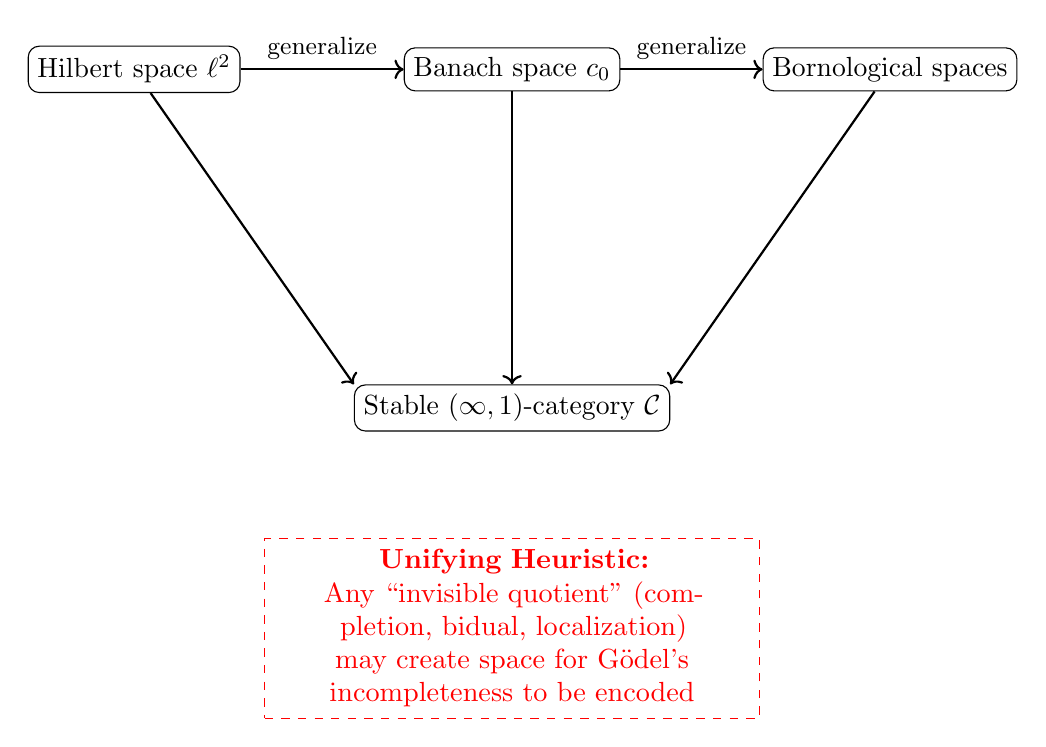
\begin{tikzpicture}[node distance=4.8 cm]
 % Top row - concrete
 \node[draw, rounded corners] (hilbert) {Hilbert space $\ell^2$};
 \node[draw, rounded corners, right of=hilbert] (banach) {Banach space $c_0$};
 \node[draw, rounded corners, right of=banach] (bornological) {Bornological spaces};
 
 % Bottom row - abstract
 \node[draw, rounded corners, below of=banach, yshift=0.5cm] (inftycat) {Stable $(\infty,1)$-category $\mathcal{C}$};
 
 % Arrows showing generalization
 \draw[->, thick] (hilbert) -- (banach) node[midway, above] {\small generalize};
 \draw[->, thick] (banach) -- (bornological) node[midway, above] {\small generalize};
 \draw[->, thick] (hilbert) -- (inftycat.north west);
 \draw[->, thick] (banach) -- (inftycat);
 \draw[->, thick] (bornological) -- (inftycat.north east);
 
 % Key insight box
 \node[draw, dashed, red, below of=inftycat, yshift=2 cm, text width=6cm, align=center, inner sep=4pt] (principle) {
    \textbf{Unifying Heuristic:}\\
    Any ``invisible quotient'' (com-\\
    pletion, bidual, localization)\\
    may create space for Gödel's\\
    incompleteness to be encoded
 };
\end{tikzpicture}
\caption{The Gödel--Banach correspondence generalizes from concrete Hilbert spaces to abstract stable $(\infty,1)$-categories. The undecidability mechanism is not tied to any particular model but reflects a deep structural principle.}
\label{fig:generalization}
\end{figure}

\paragraph{Data and code availability.}
Lean 4 source files are hosted at
\url{https://github.com/AICardiologist/FoundationRelativity}.
Snapshot \leanRepoTag{} contains the complete formalization with 0 sorries.
\llmNote

\paragraph{Acknowledgments.}
I thank \textbf{Emily Riehl} for the inspiration provided by her 2025
London Mathematical Society \emph{Hardy Lectures}, whose bicategorical
perspective influenced the present work. The Lean formalization community and AI assistants provided crucial insights during the mechanization process.

% ============================================================

\bibliographystyle{amsalpha}
\begin{thebibliography}{99}
\bibitem{Atk51}
F.~V. Atkinson. ``The normal solvability of linear equations in normed spaces.'' \emph{Mat. Sbornik N.S.}, 28(70) (1951), 3--14.
\bibitem{BR87}
D. Bridges and F. Richman. \emph{Varieties of Constructive Mathematics.} Cambridge University Press, 1987.
\bibitem{Bri94a}
D. Bridges. ``Constructive functional analysis: a survey.'' \emph{Quaestiones Mathematicae}, 17(3) (1994), 305--322.
\bibitem{CS09}
T. Coquand and B. Spitters. ``Formalizing constructive Gelfand duality.'' \emph{Mathematical Proceedings of the Cambridge Philosophical Society}, 147(2) (2009), 339--354.
\bibitem{CPGW15}
T.~S. Cubitt, D. Perez-Garcia, and M.~M. Wolf. ``Undecidability of the spectral gap.'' \emph{Nature,} 528(7581) (2015), 207--211.
\bibitem{DL84}
J. Denef and L. Lipshitz. ``Power series solutions of algebraic differential equations.'' \emph{Mathematische Annalen,} 267 (1984), 213--238.
\bibitem{GohbergKrein}
I.~C. Gohberg and M.~G. Krein. \emph{Introduction to the Theory of Linear Nonselfadjoint Operators.} AMS, 1969.
\bibitem{Hog77}
H. Hogbe-Nlend. \emph{Bornologies and Functional Analysis.} North-Holland, 1977.
\bibitem{Joh02}
P.~T. Johnstone. \emph{Sketches of an Elephant: A Topos Theory Compendium}, Vols. 1--2. Oxford University Press, 2002.
\bibitem{Kar94}
J. Kari. ``Reversibility and surjectivity problems of cellular automata.'' \emph{Journal of Computer and System Sciences,} 48(1) (1994), 149--182.
\bibitem{Kato}
T. Kato. \emph{Perturbation Theory for Linear Operators.} Springer, 1995.
\bibitem{Kaye94}
R. Kaye. \emph{Models of Peano Arithmetic.} Oxford University Press, 1991.
\bibitem{Lur09}
J. Lurie. \emph{Higher Topos Theory.} Princeton University Press, 2009.
\bibitem{LurieHA}
J. Lurie. \emph{Higher Algebra.} Available at \url{https://www.math.ias.edu/~lurie/}, 2017.
\bibitem{Mey99}
R. Meyer. ``Bornological versus topological analysis in metrizable spaces.'' \emph{Contemporary Mathematics,} 289 (2001), 249--278.
\bibitem{PER89}
M. B. Pour-El and J. I. Richards. \emph{Computability in Analysis and Physics.} Springer, 1989.
\bibitem{Pro00}
F. Prosmans. ``Derived categories for functional analysis.'' \emph{Publications of the RIMS,} 36 (2000), 19--83.
\bibitem{RV22}
E.~Riehl and D.~Verity. \emph{Elements of $\infty$-Category Theory.}
Cambridge University Press, 2022.
\bibitem{TD88}
A.~S. Troelstra and D. van Dalen. \emph{Constructivism in Mathematics, Vol. I.} North-Holland, 1988.
\bibitem{UFP13}
The Univalent Foundations Program. \emph{Homotopy Type Theory: Univalent Foundations of Mathematics.} Institute for Advanced Study, 2013.


\end{thebibliography}
\end{document}